\chapter{Lidar odometry (step 1)}
This software calculates trajectory based on Lidar and IMU data.
It based on novel approach that I did not have opportunity to publish (work in progress).
Basically it is SAM (Smoothing and Mapping) approach that is using multi view Normal Distributions Transform in pose graph SLAM framework writen from scratch in Python (SymPy) and C++ (Eigen).
 

\begin{figure}
	\centering
	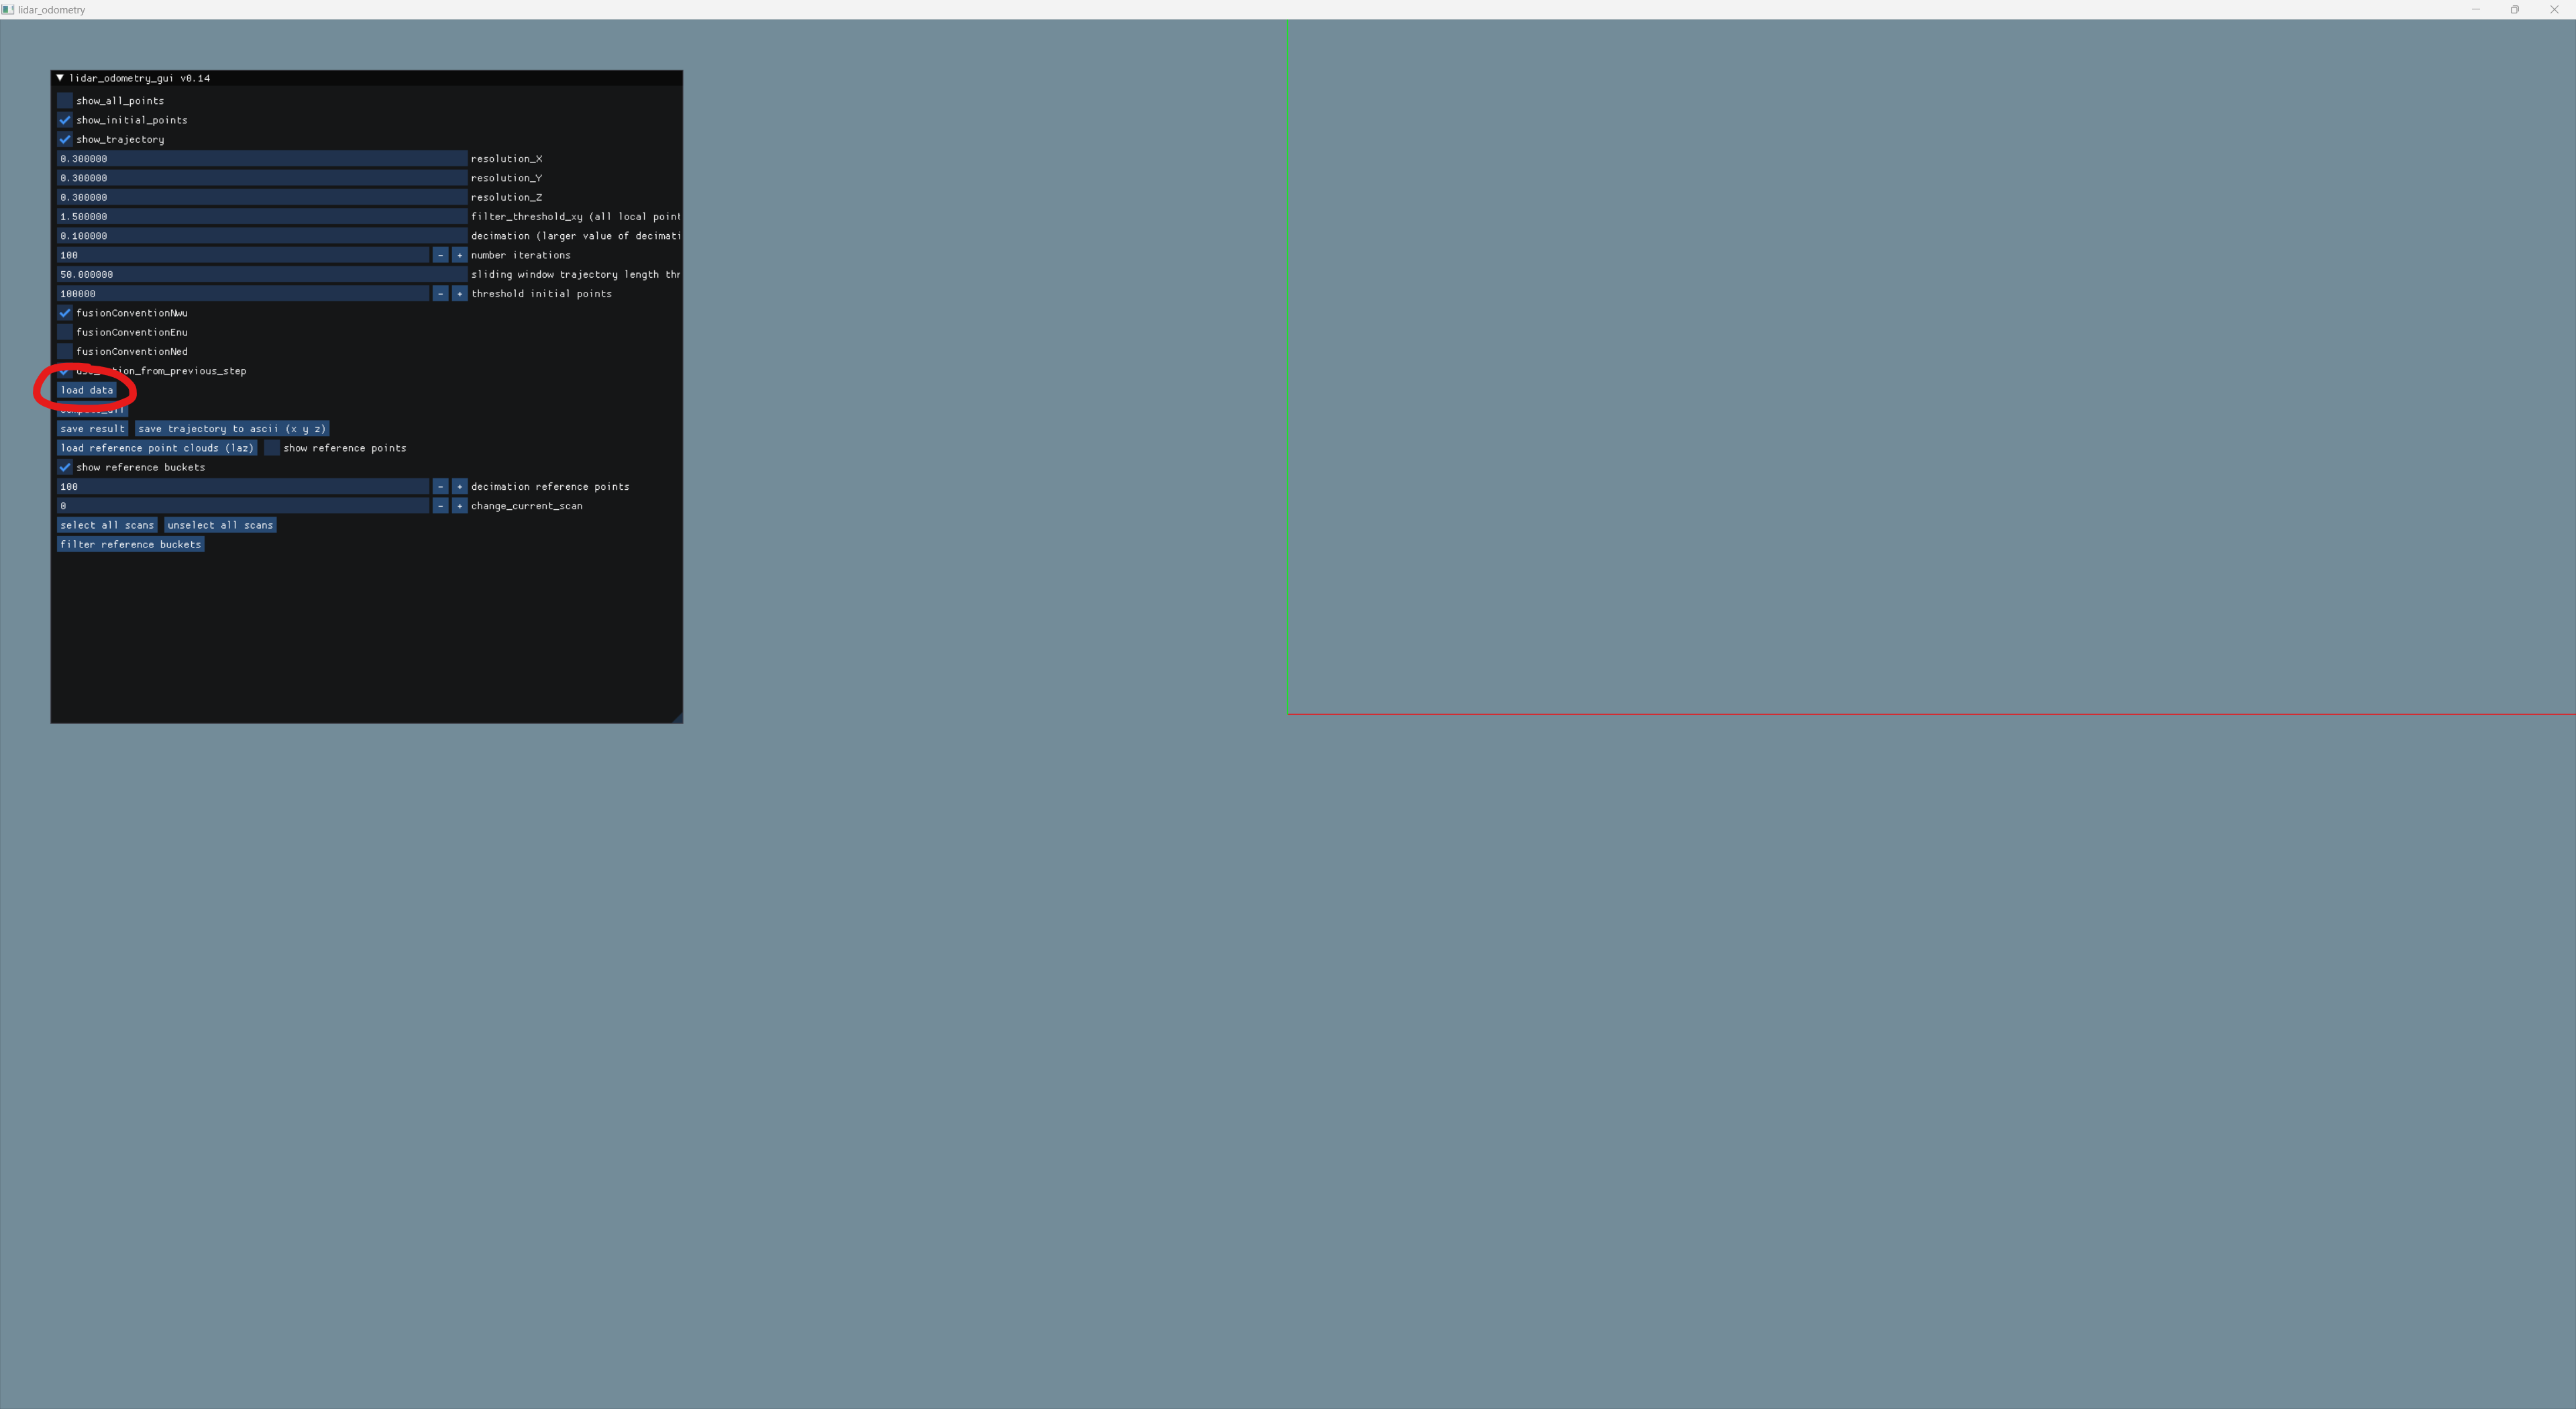
\includegraphics[width=\textwidth]{1.png}
	\caption{Step 1 - loading data.}
	\label{fig:1}
\end{figure}

\begin{figure}
	\centering
	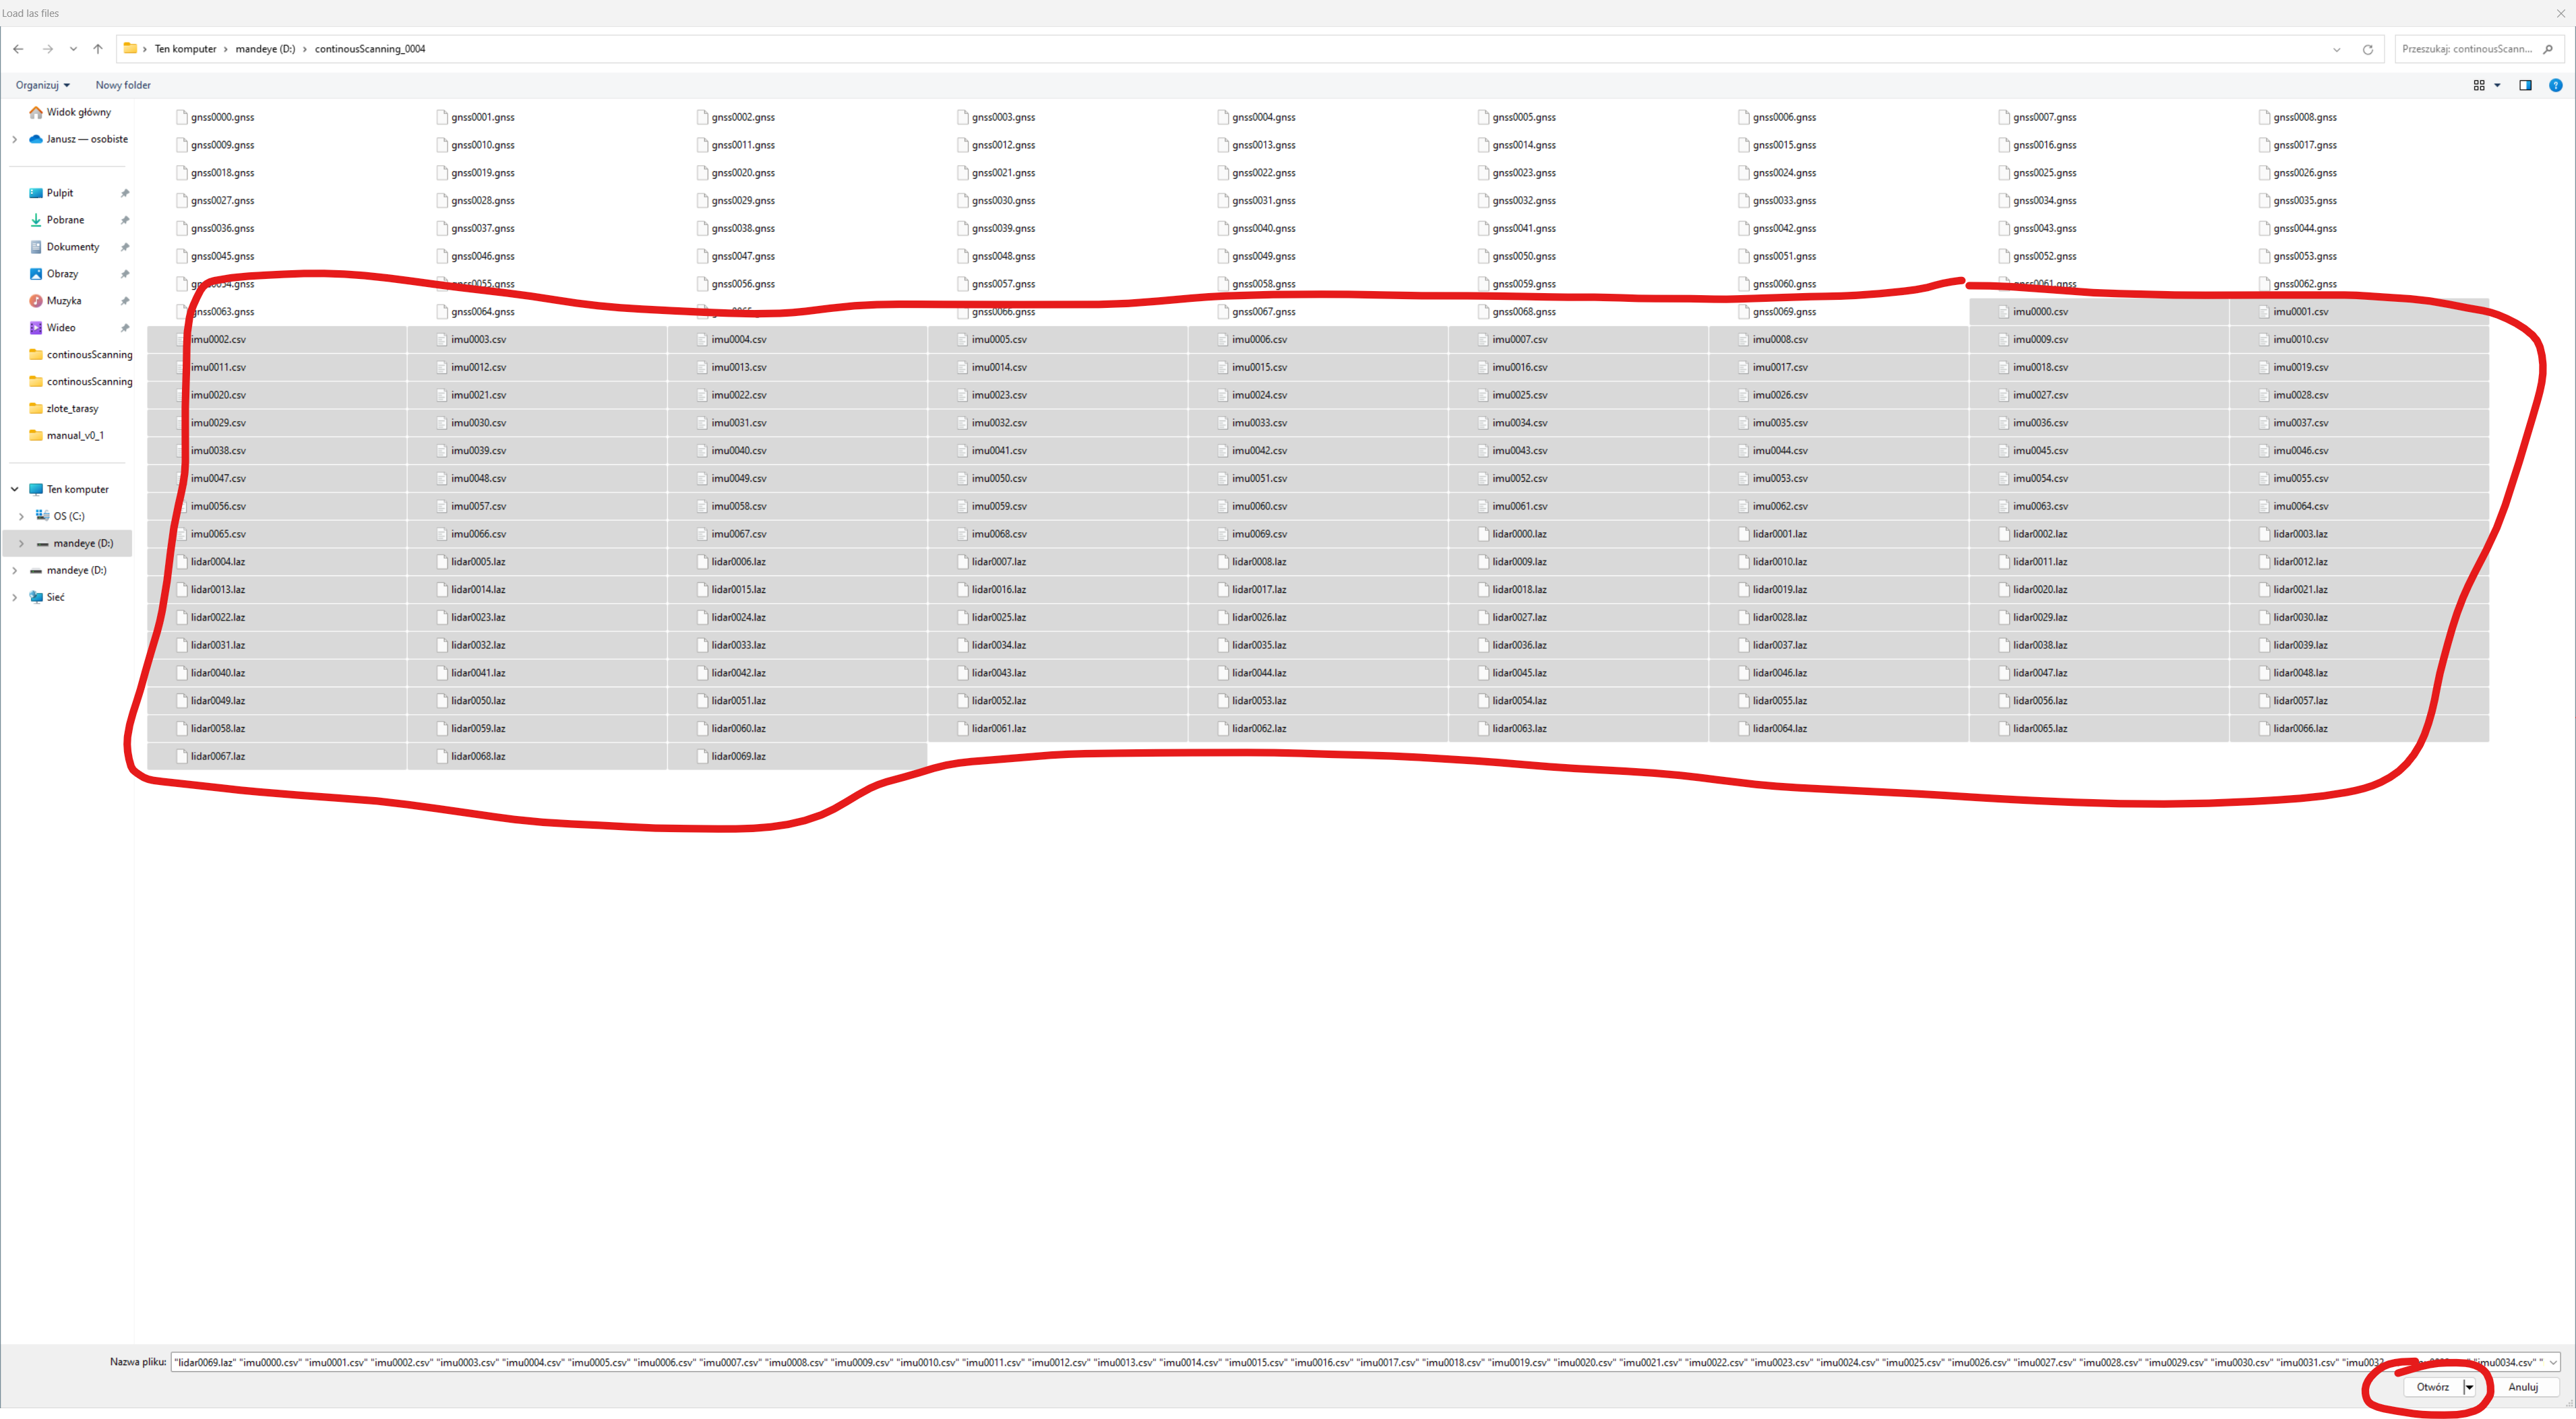
\includegraphics[width=\textwidth]{2.png}
	\caption{Step 2 - select all *.csv and *.laz files from folder that \href{https://github.com/JanuszBedkowski/mandeye_controller/blob/main/doc/manual/manual_v0_1/mandeye_dev_manual_v0_1.pdf}{MANDEYE} mobile mapping system created on USB drive.}
	\label{fig:2}
\end{figure}

\begin{figure}
	\centering
	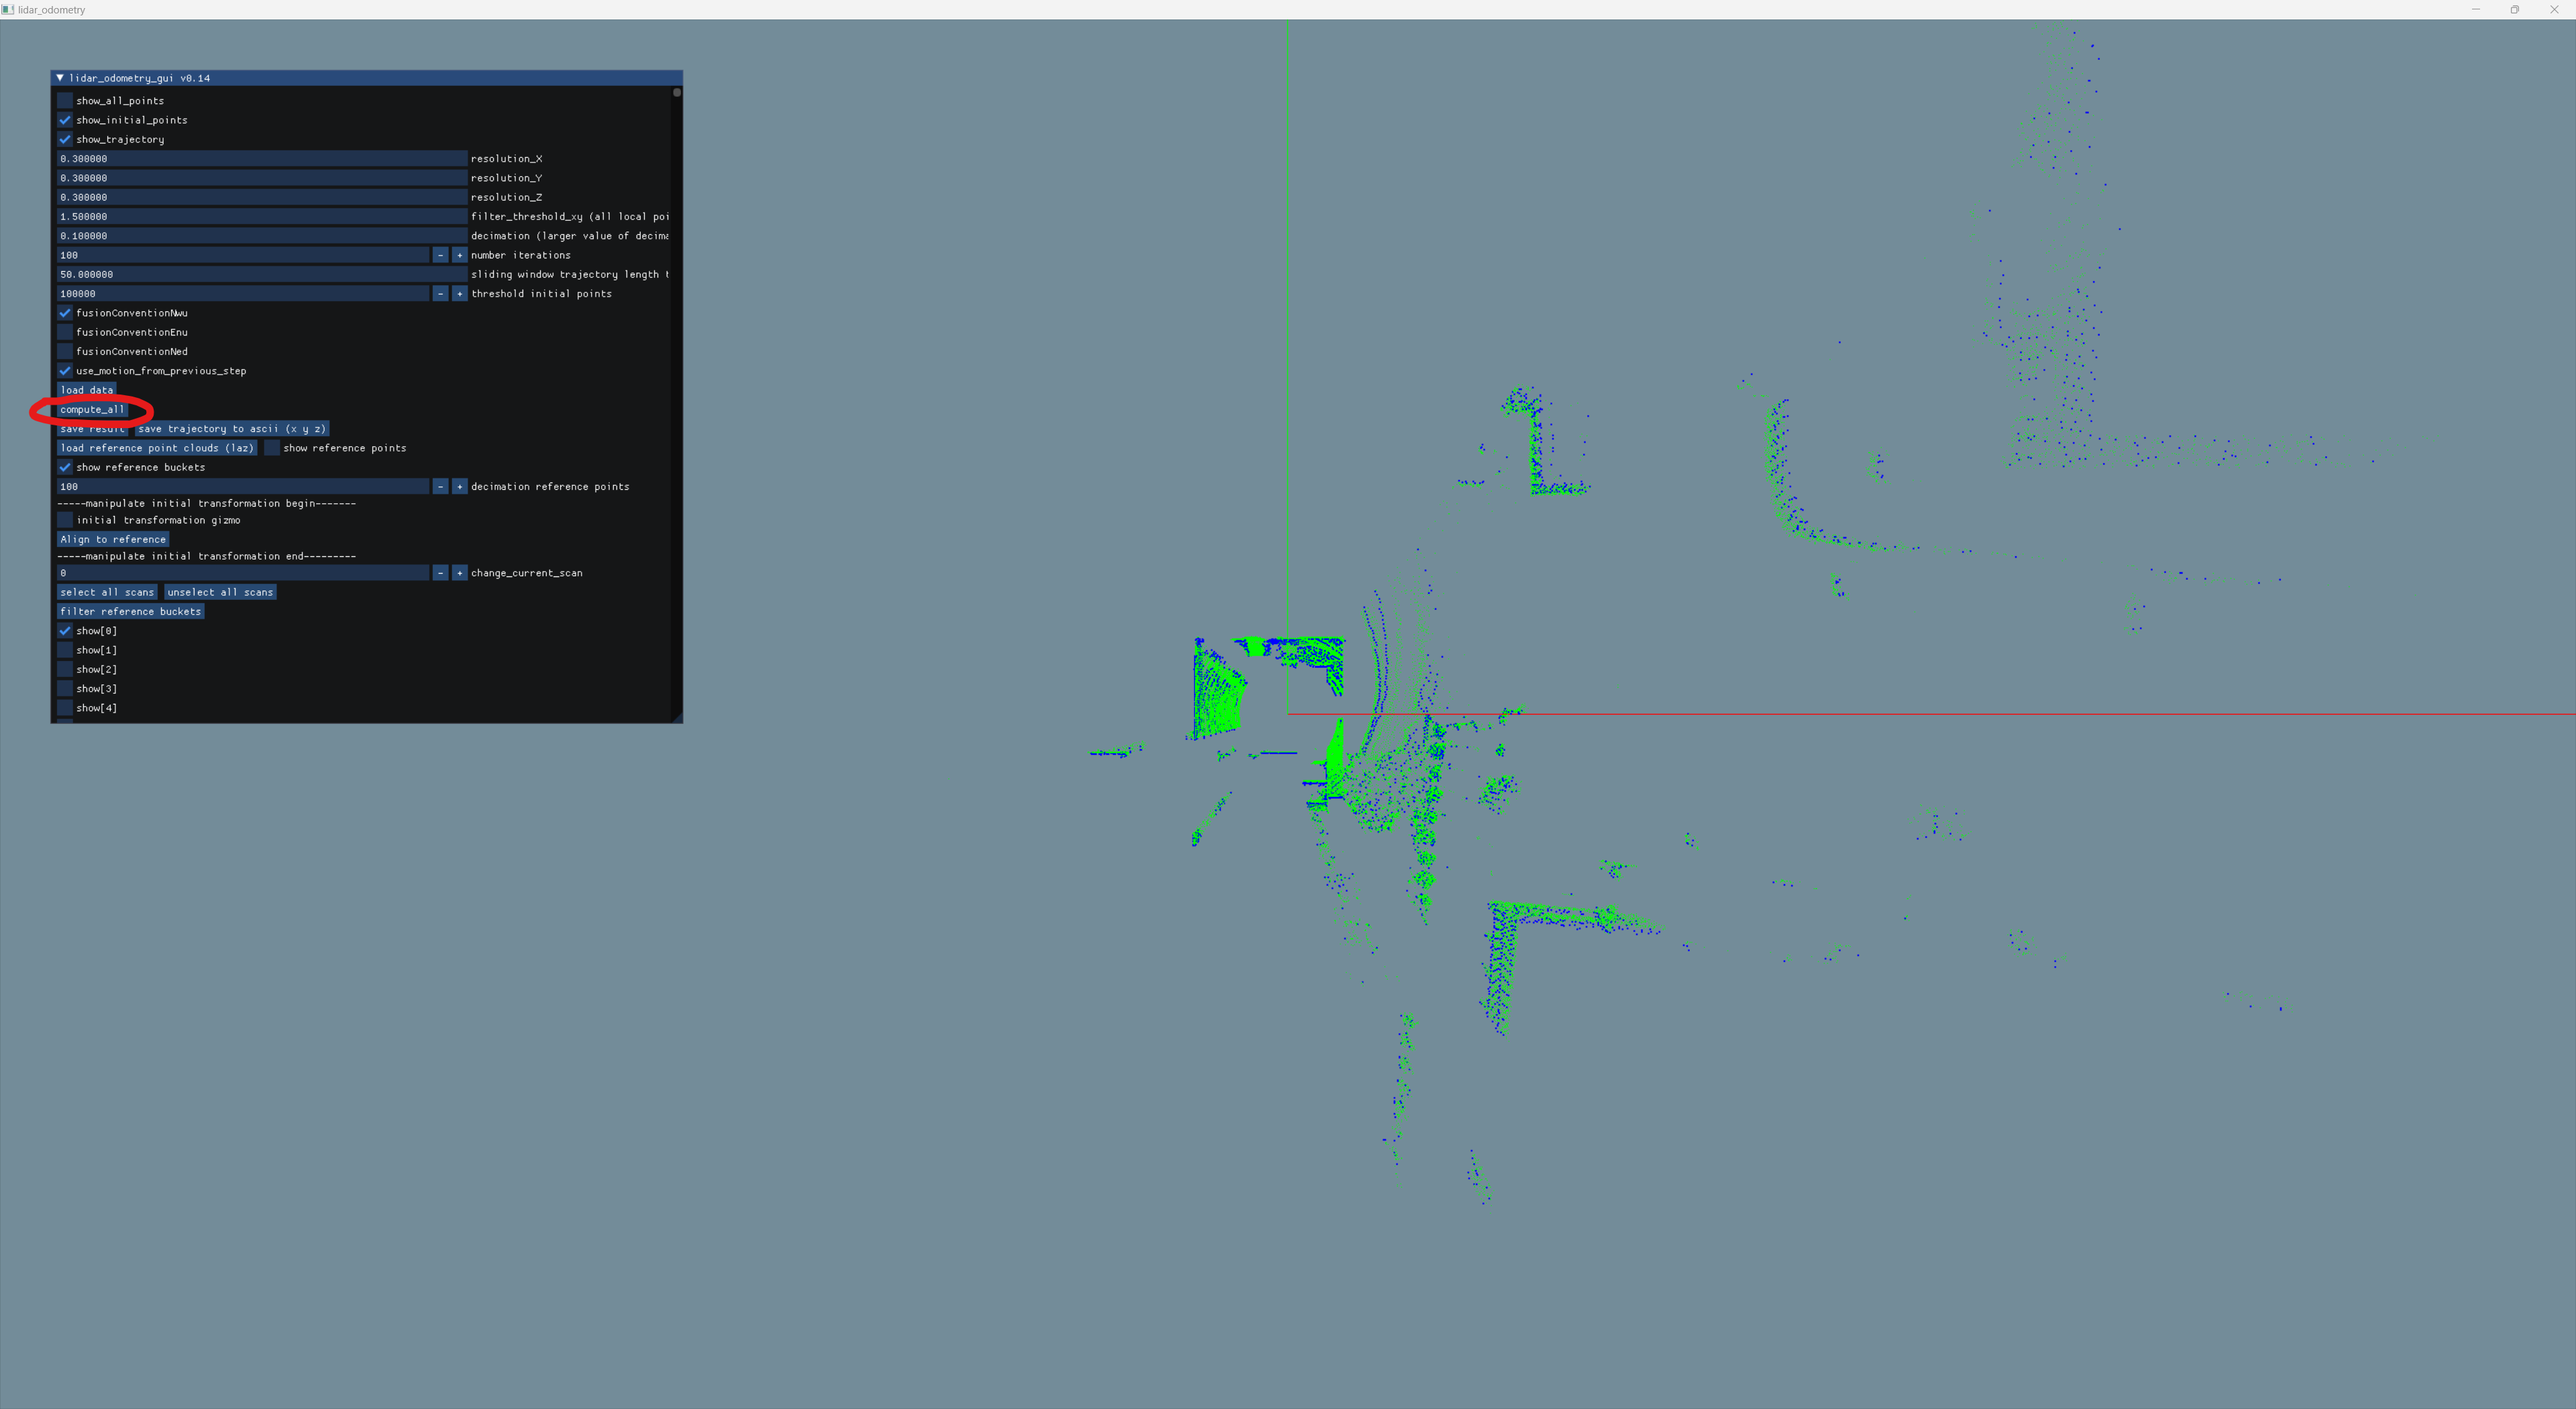
\includegraphics[width=\textwidth]{3.png}
	\caption{Step 3 - press 'compute all'. Check console mean time and folder 'preview'.}
	\label{fig:3}
\end{figure}

\begin{figure}
	\centering
	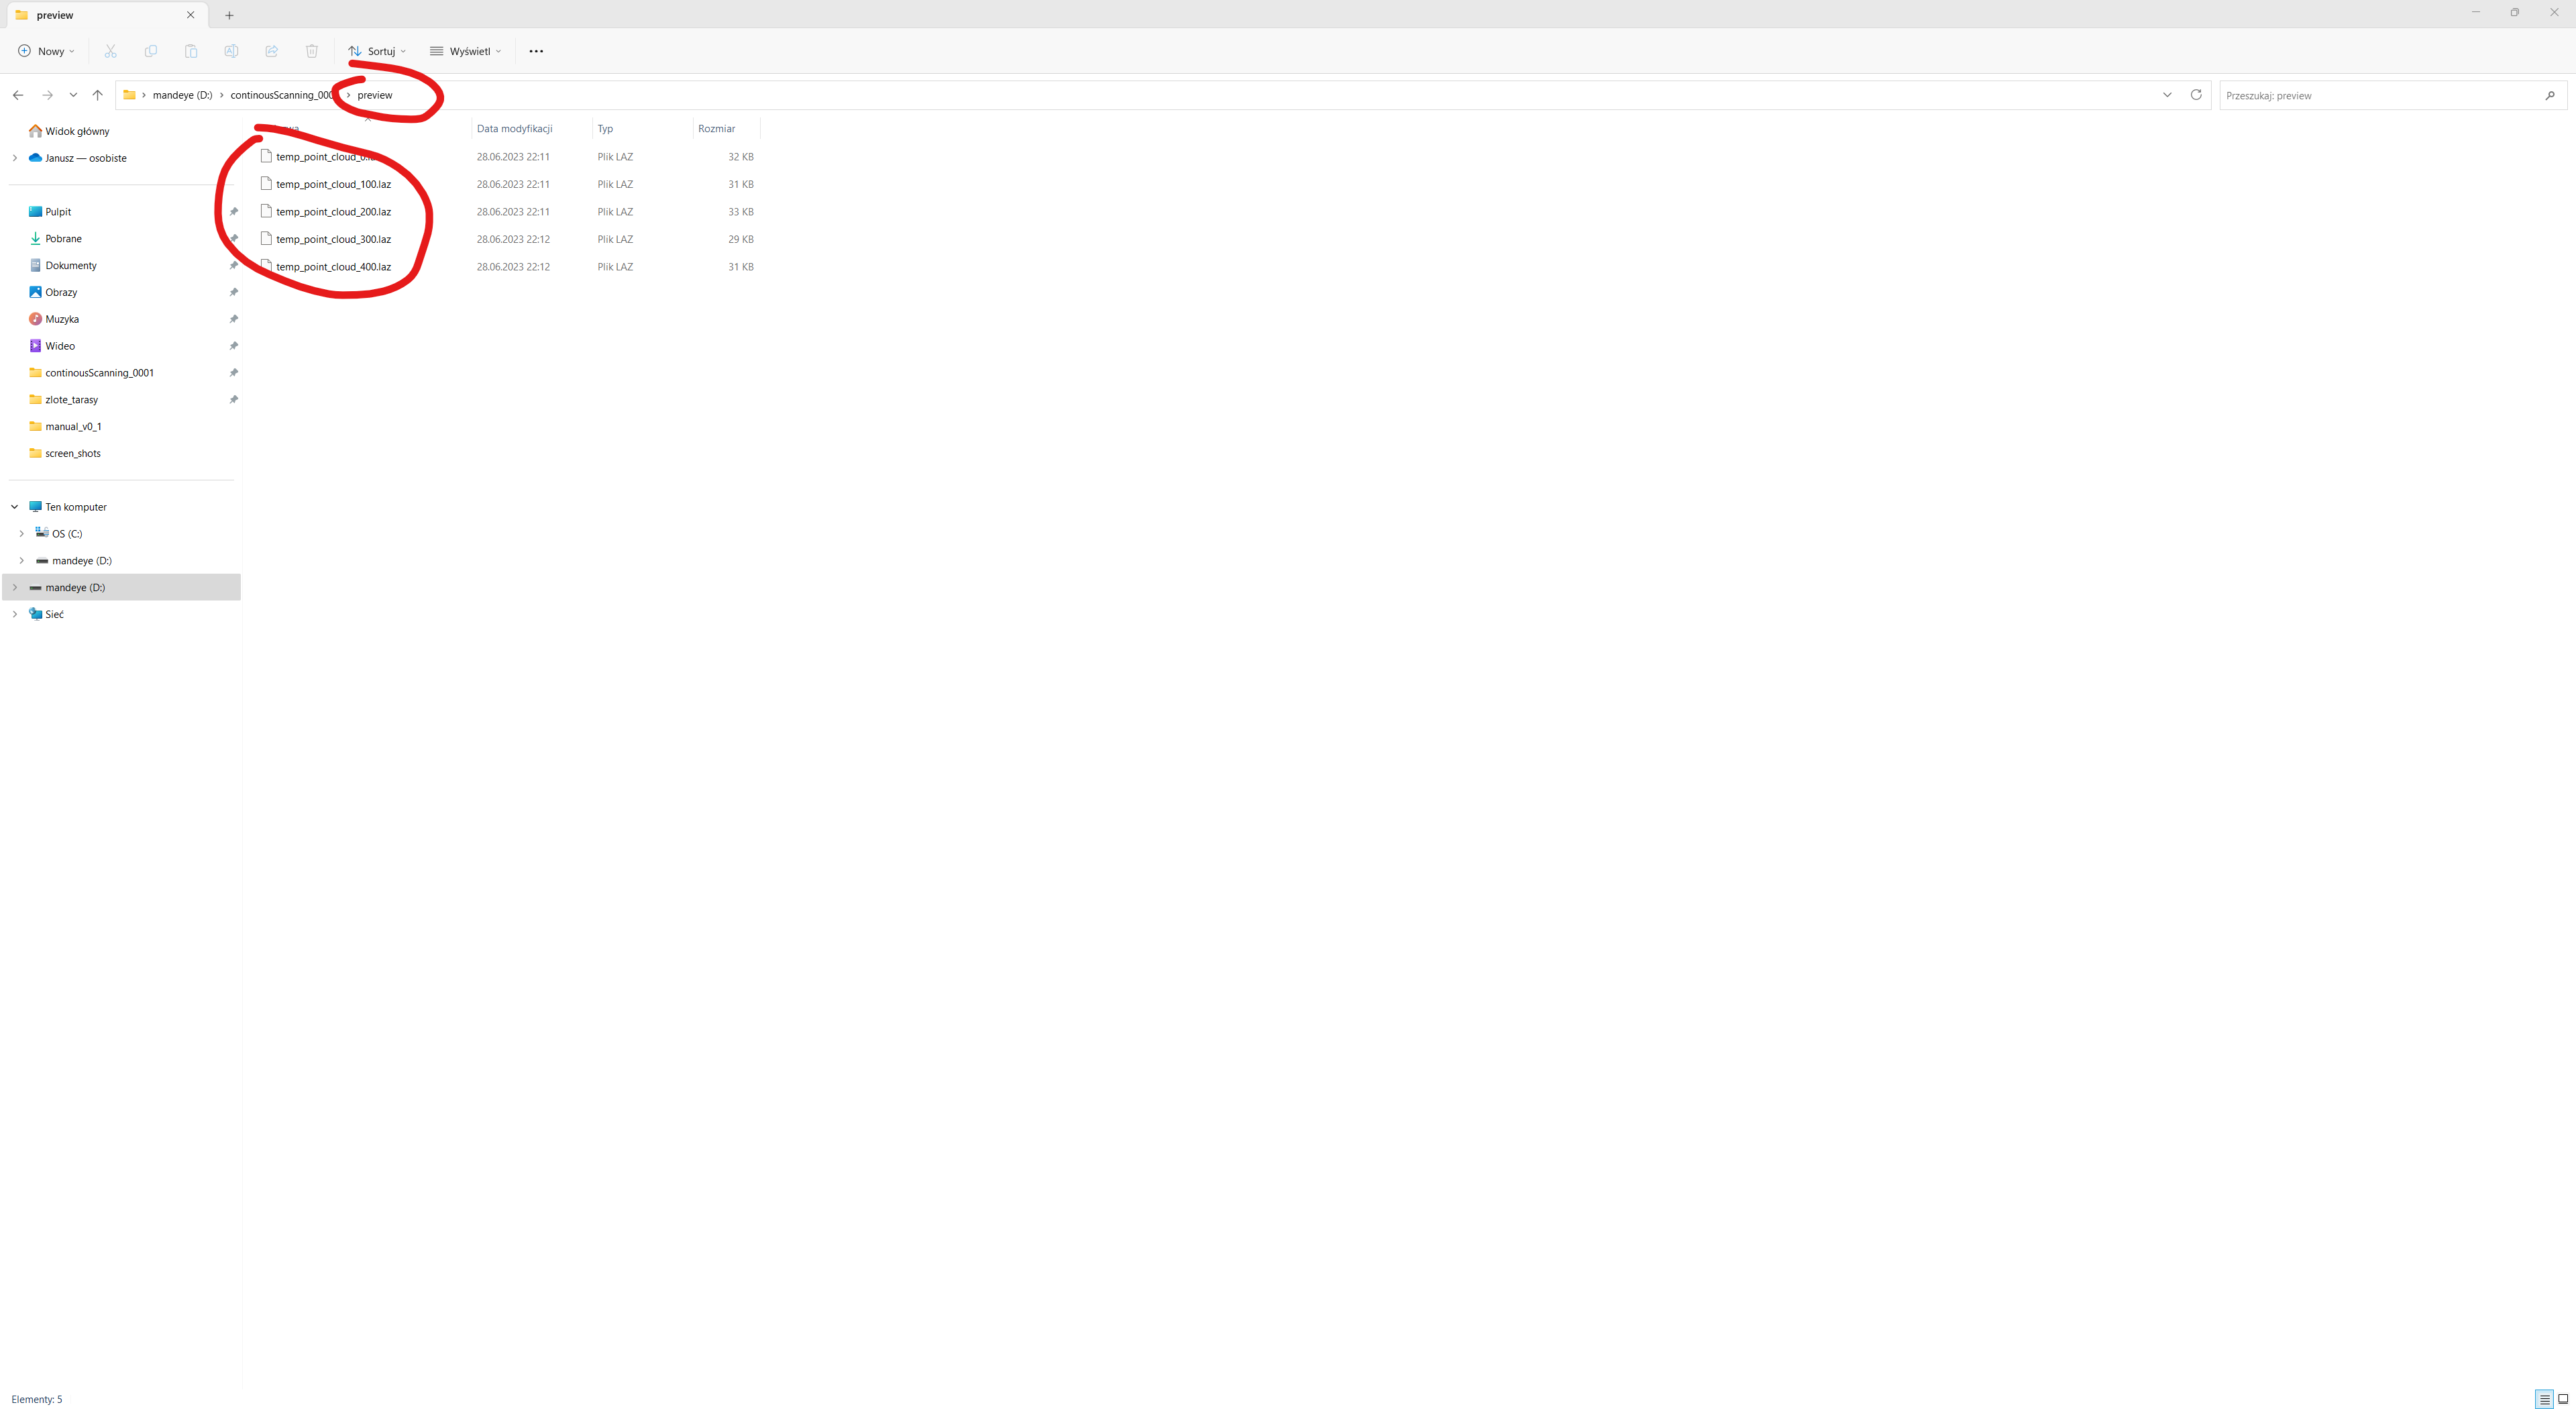
\includegraphics[width=\textwidth]{4.png}
	\caption{Optional step: intermediate results are stored in 'preview' folder.}
	\label{fig:4}
\end{figure}

\begin{figure}
	\centering
	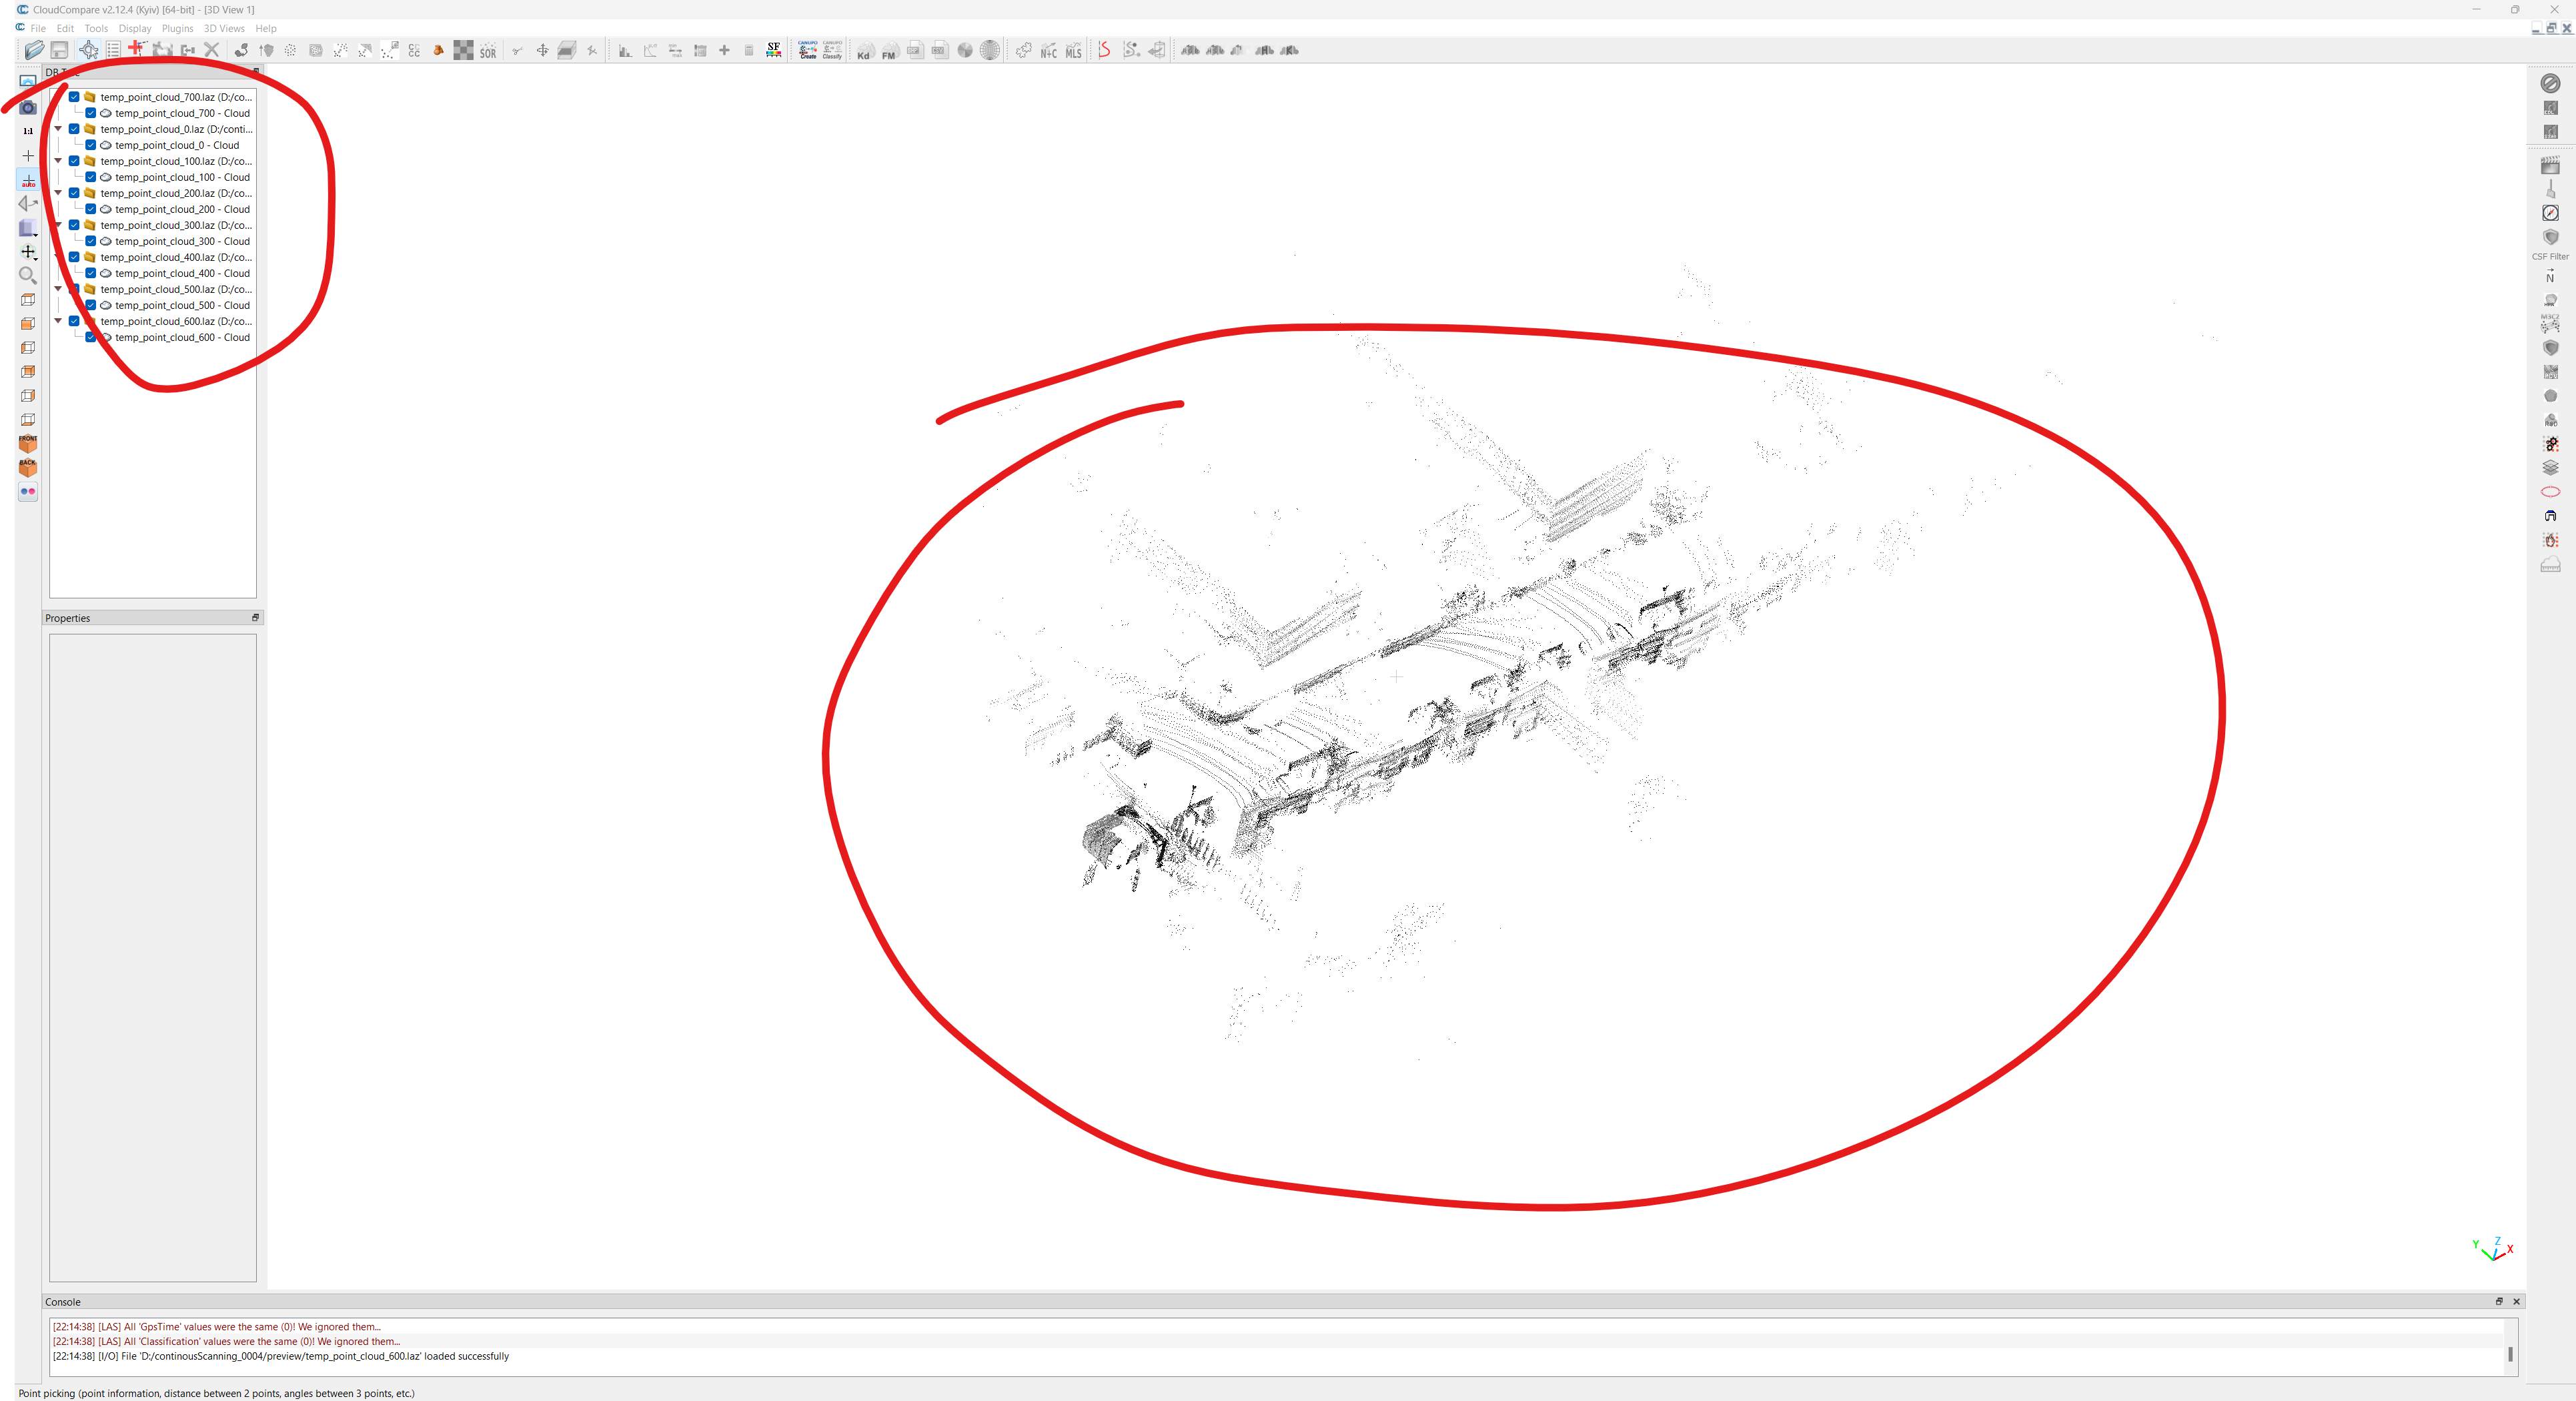
\includegraphics[width=\textwidth]{5.png}
	\caption{Optional step: You can watch the progress in open source \href{https://www.cloudcompare.org/}{CloudCompare} software by loading all *.laz files from 'preview' folder.}
	\label{fig:5}
\end{figure}

\begin{figure}
	\centering
	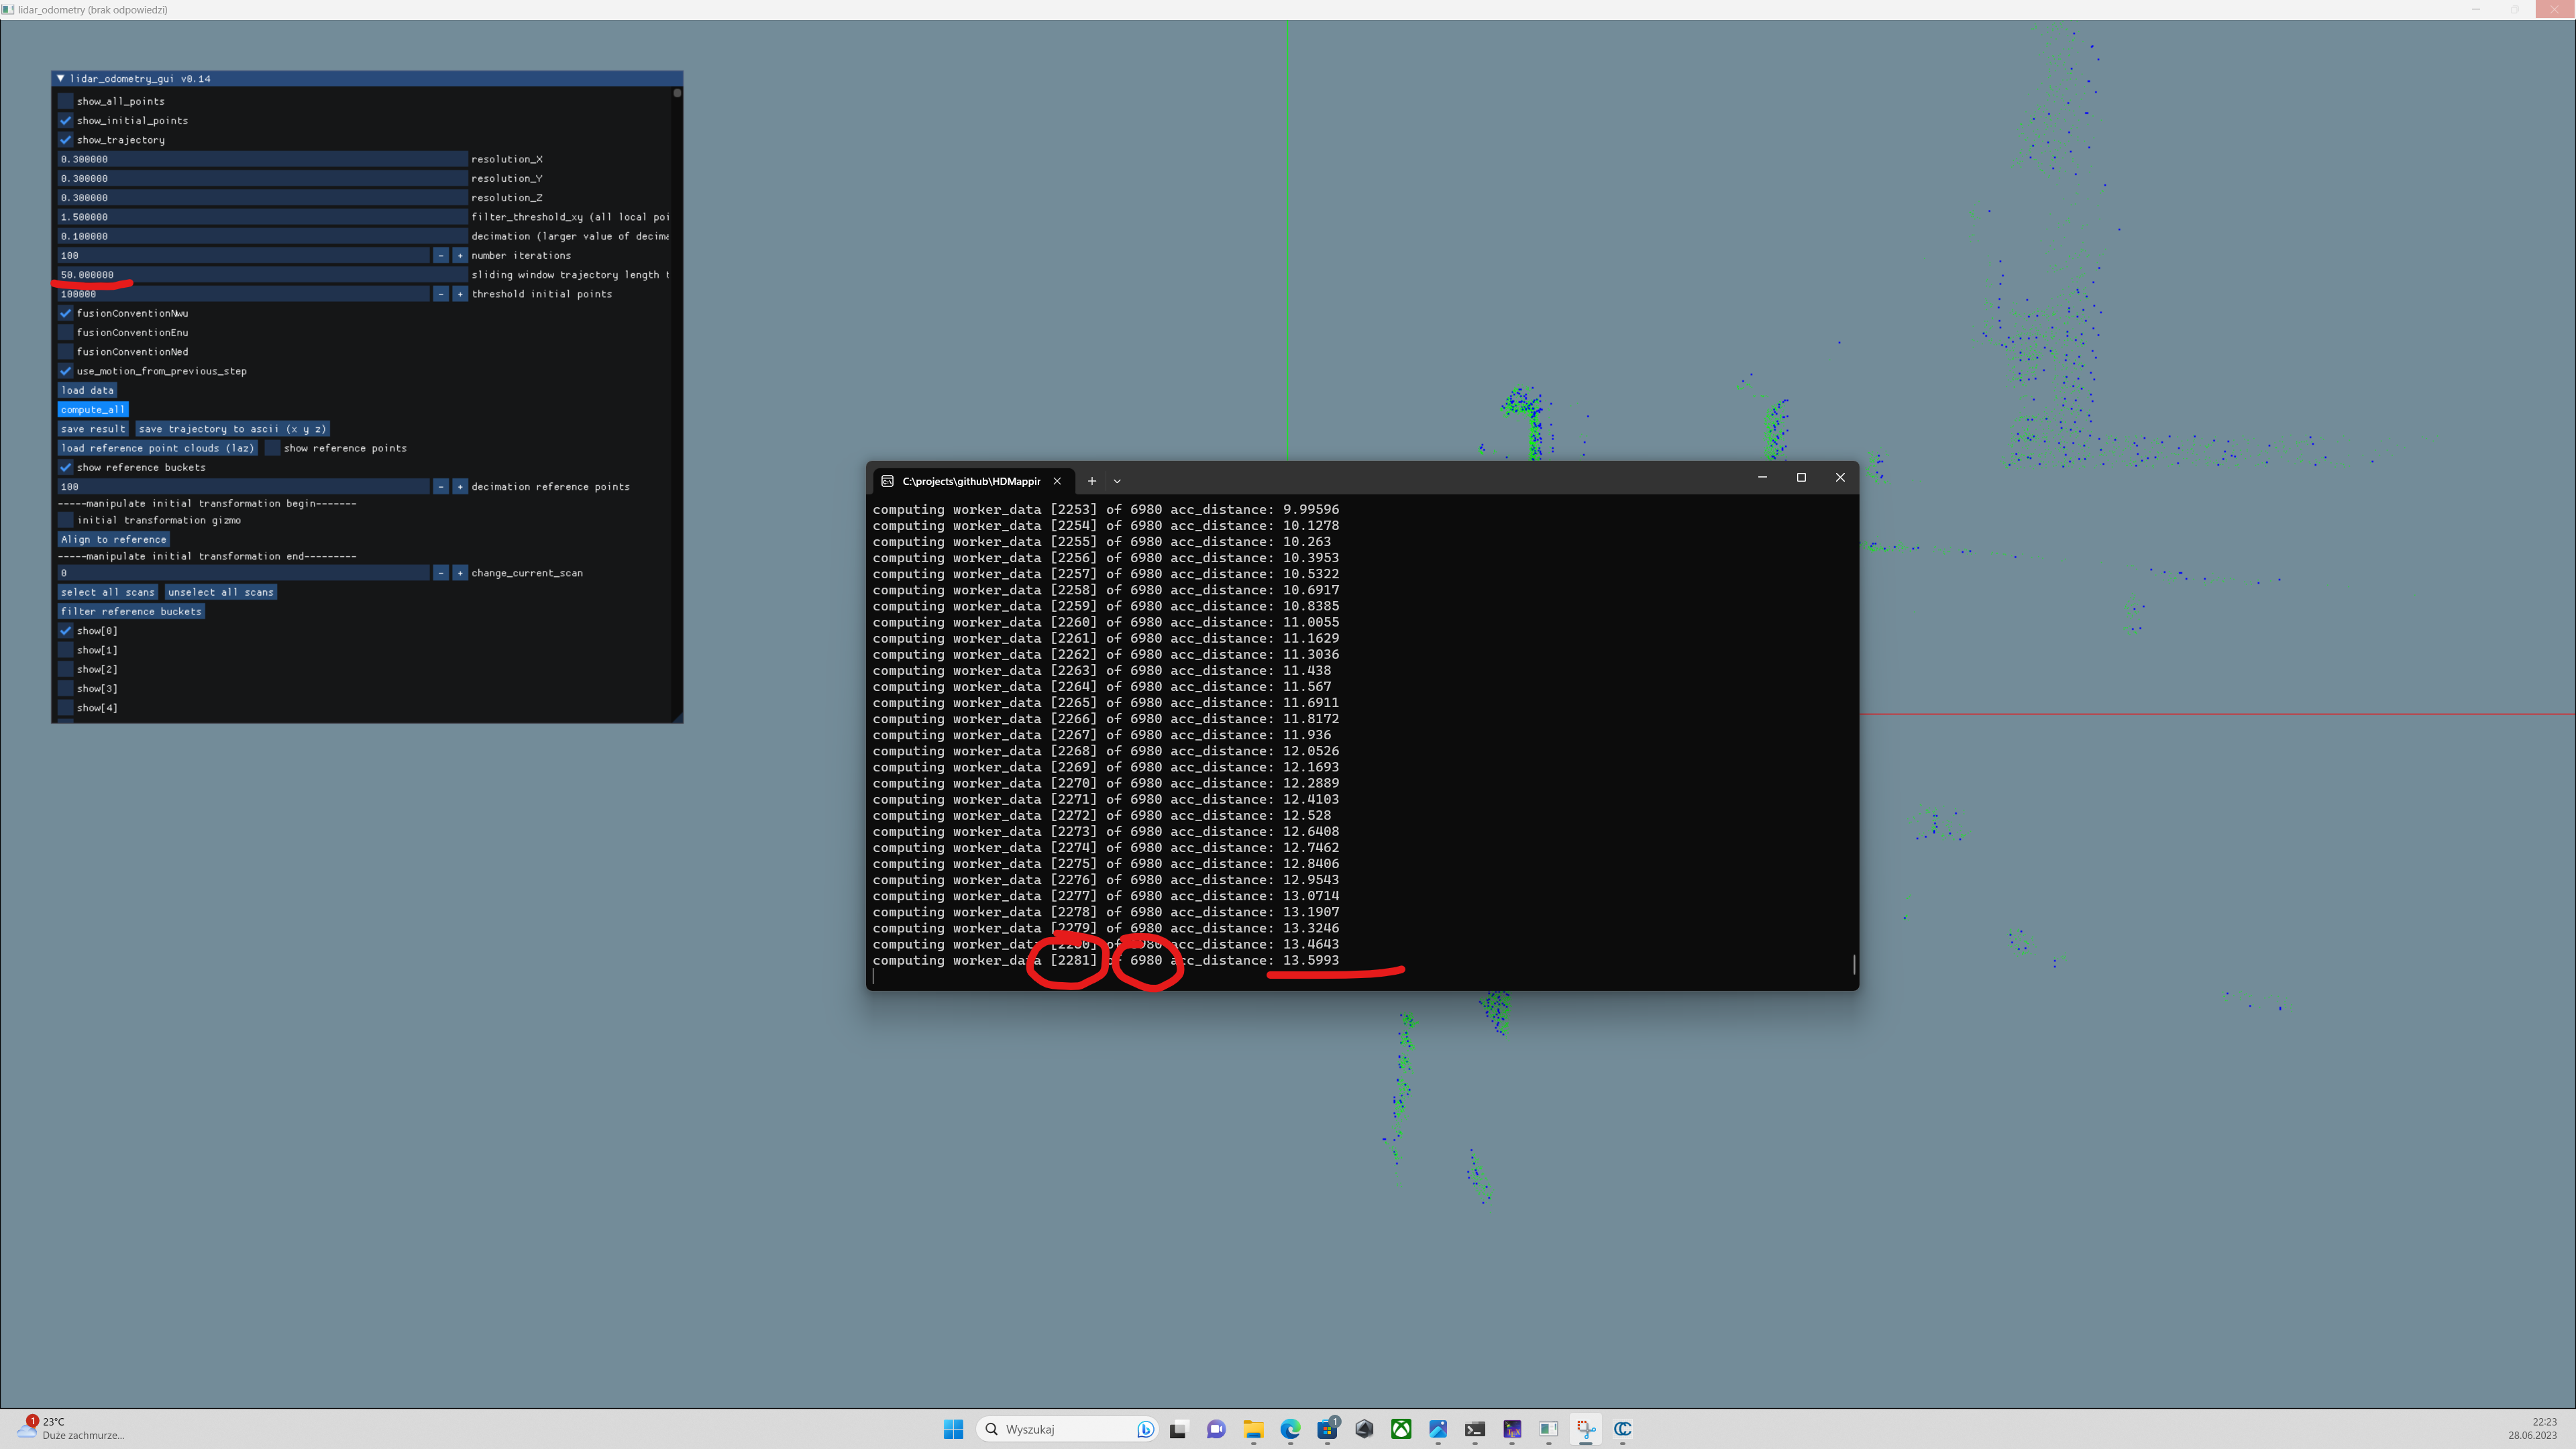
\includegraphics[width=\textwidth]{6.png}
	\caption{Progress in console.}
	\label{fig:6}
\end{figure}

\begin{figure}
	\centering
	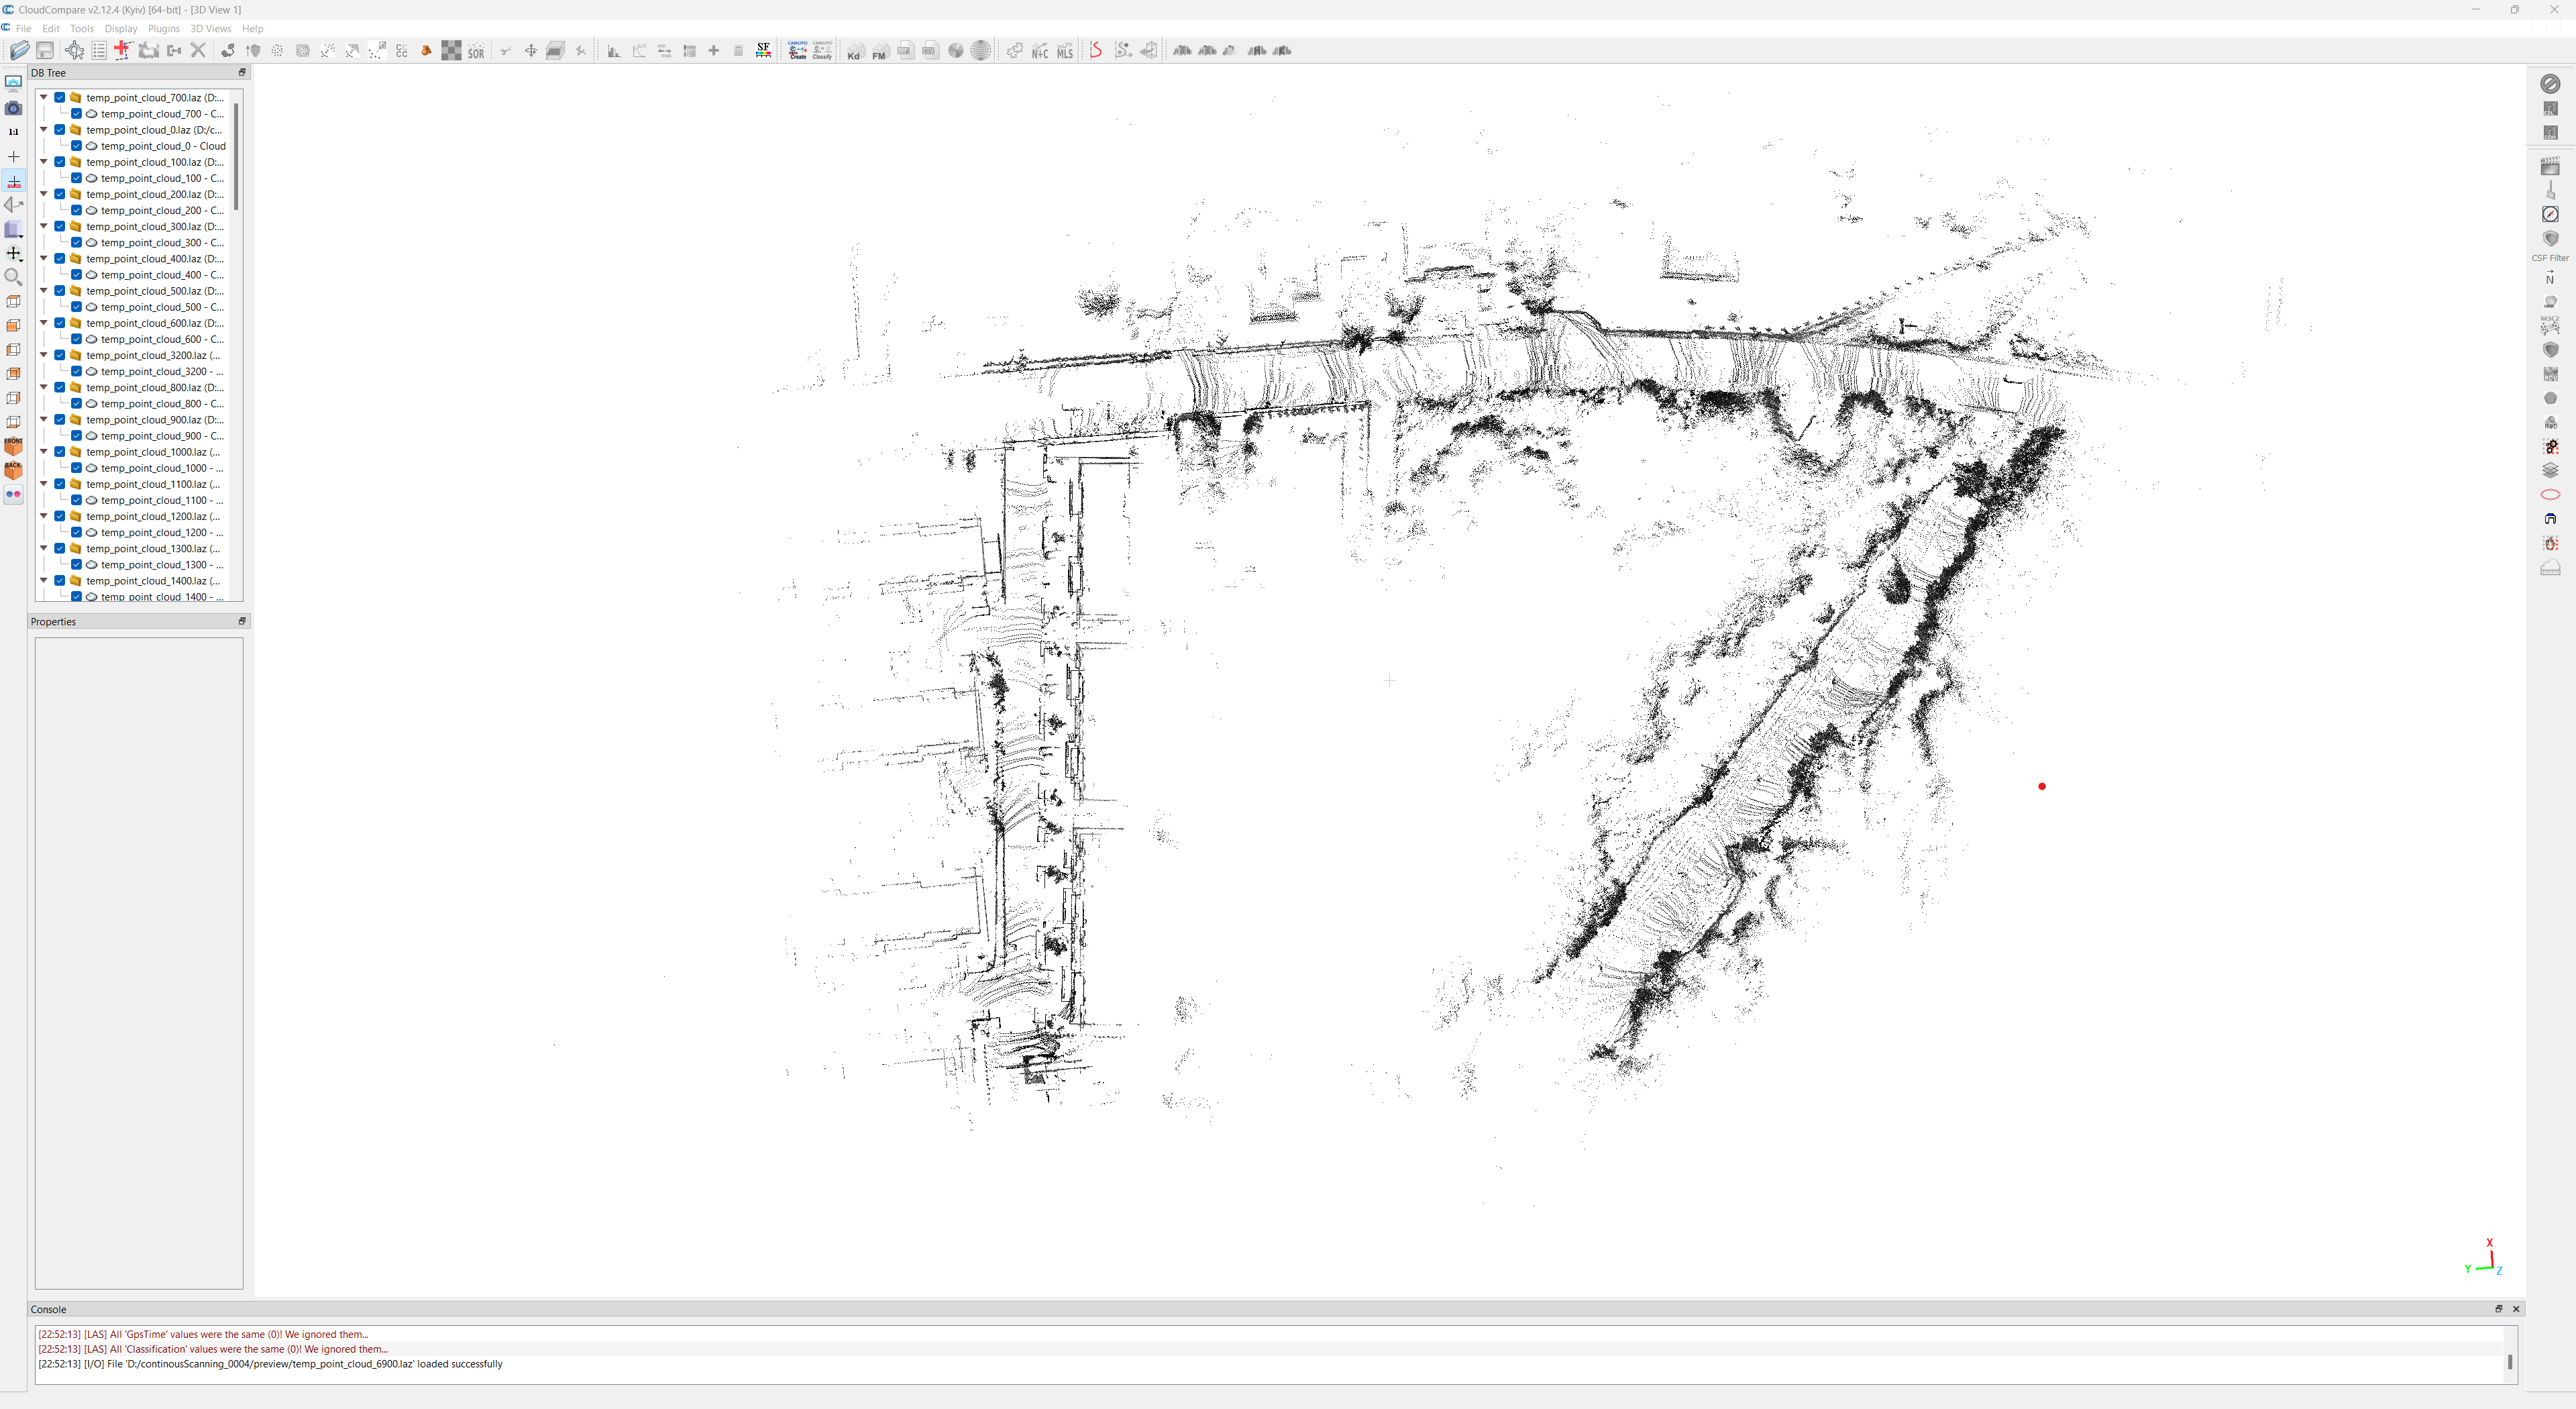
\includegraphics[width=\textwidth]{7.png}
	\caption{Final data in \href{https://www.cloudcompare.org/}{CloudCompare}.}
	\label{fig:7}
\end{figure}

\begin{figure}
	\centering
	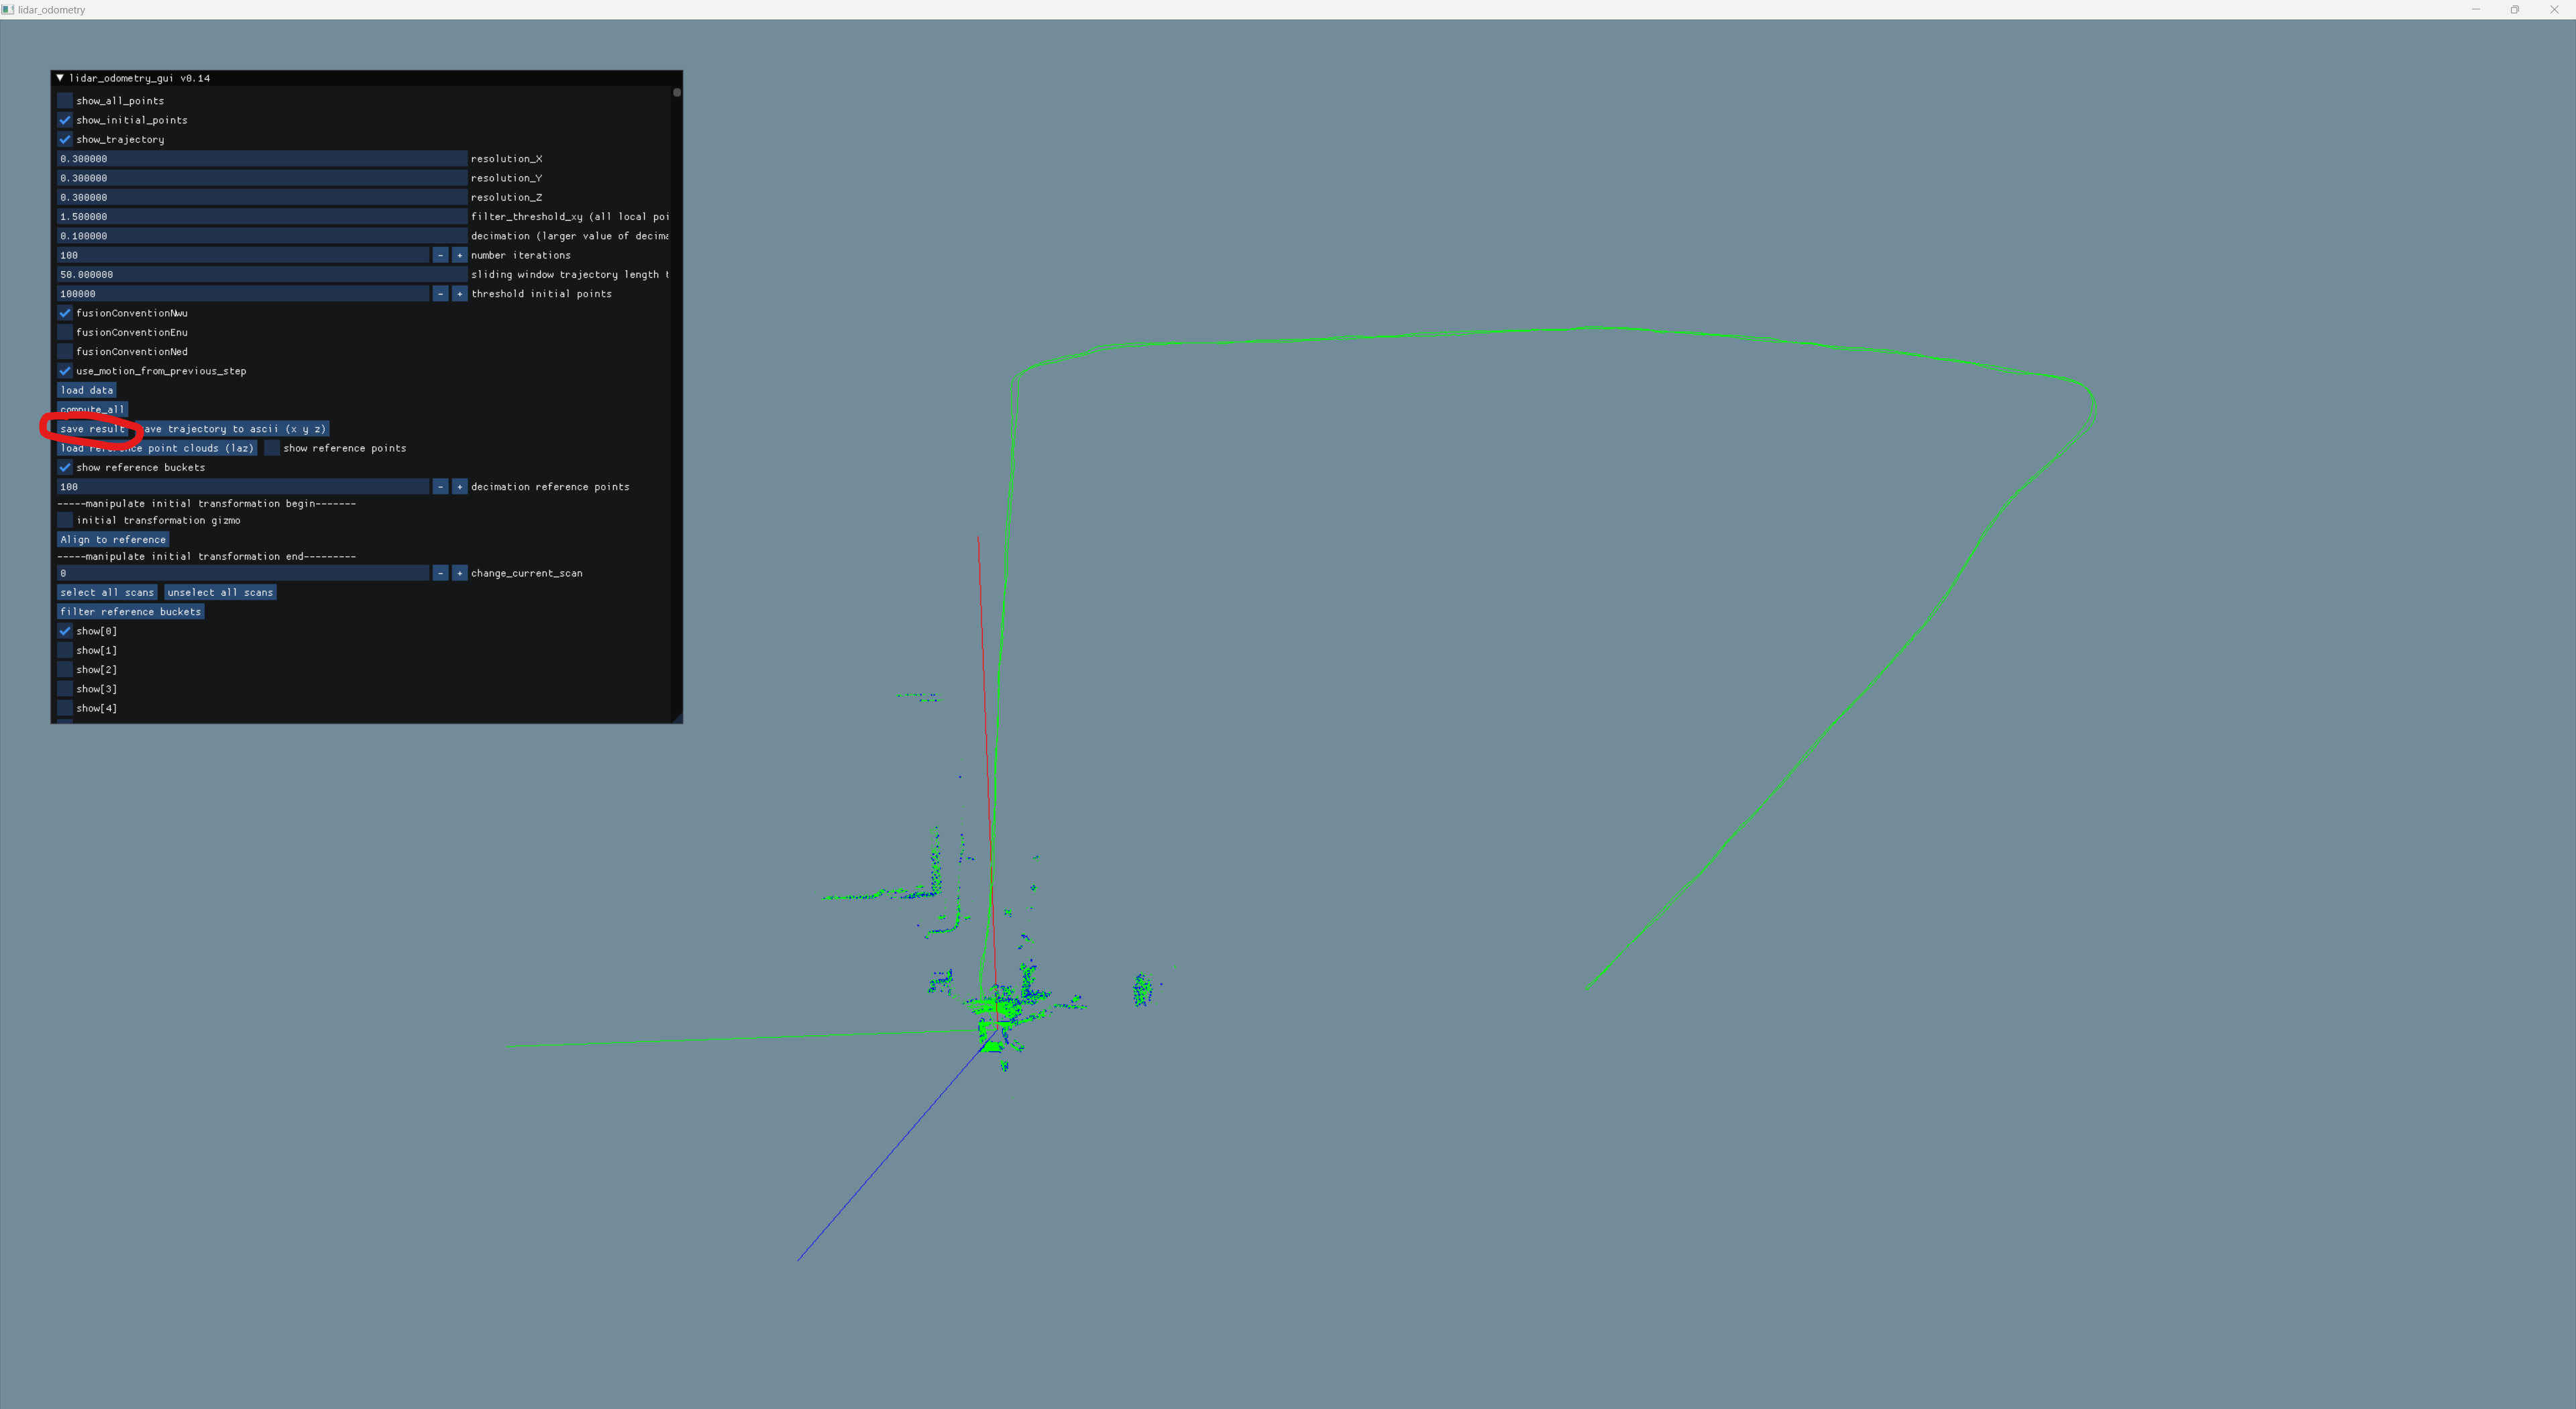
\includegraphics[width=\textwidth]{8.png}
	\caption{Final data ready for export.}
	\label{fig:8}
\end{figure}

\begin{figure}
	\centering
	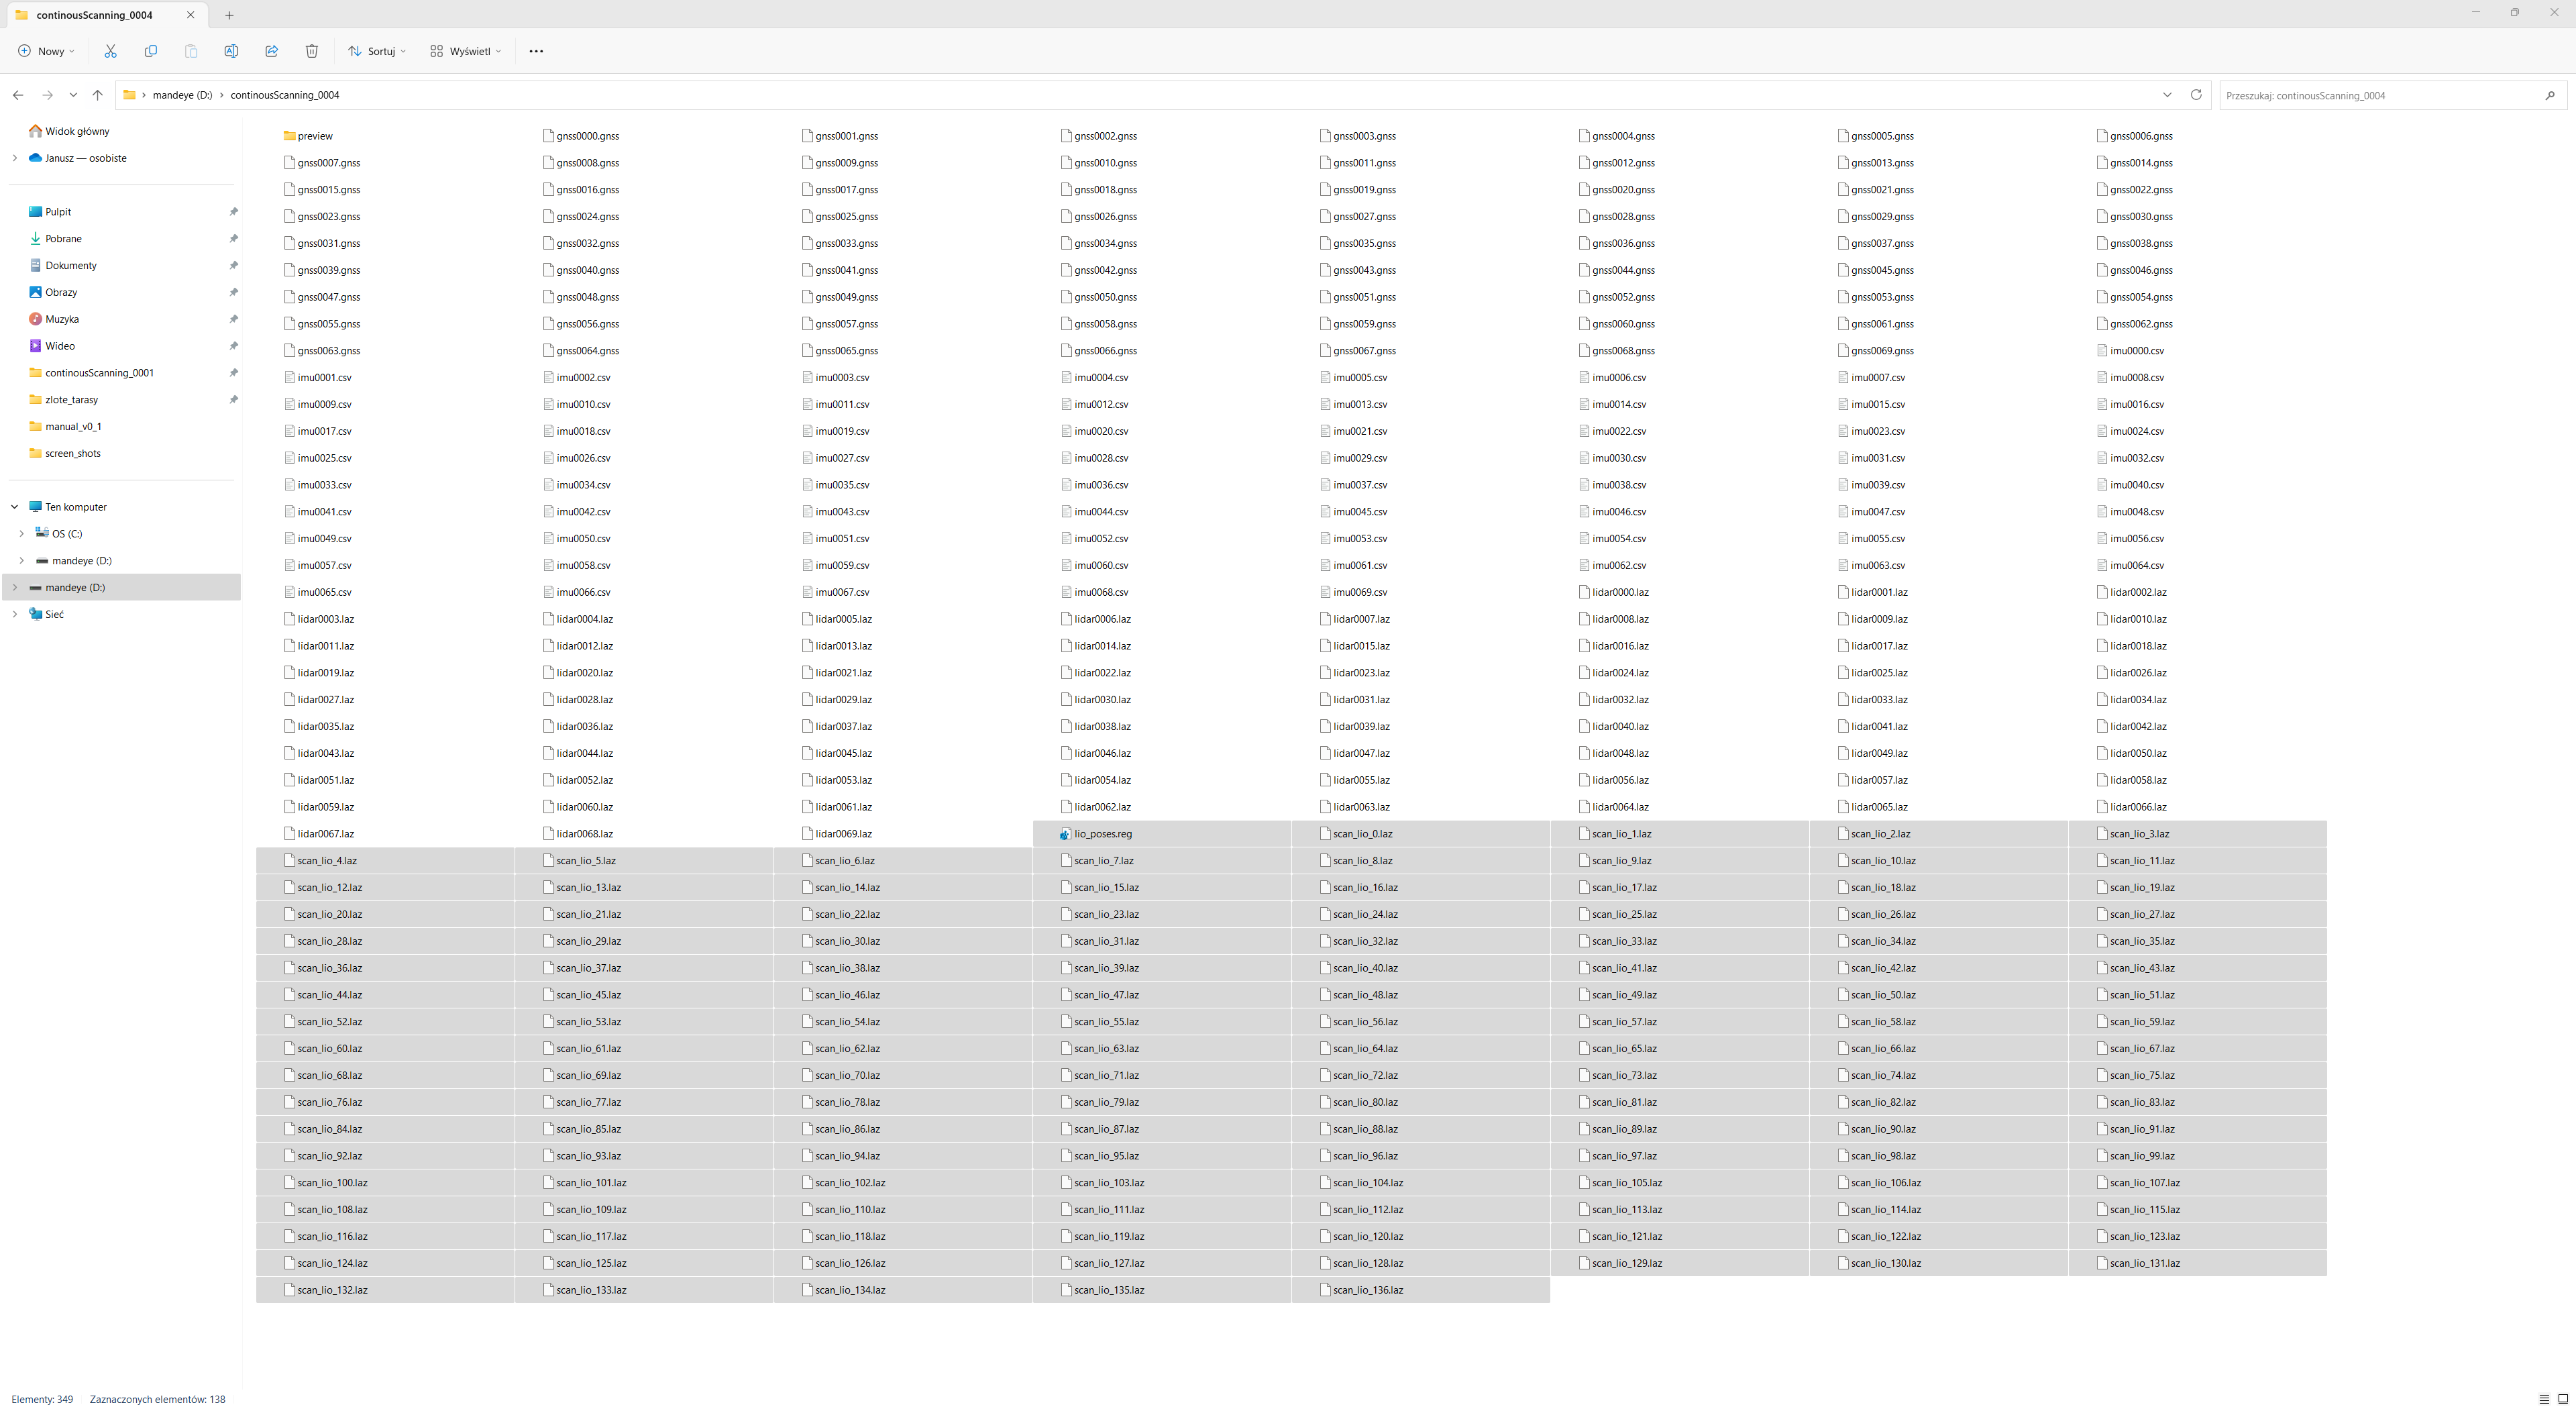
\includegraphics[width=\textwidth]{9.png}
	\caption{Exported final files.}
	\label{fig:9}
\end{figure}